\documentclass[letterpaper,10pt]{article}
\usepackage[top=2cm, bottom=1.5cm, left=1cm, right=1cm]{geometry}
\usepackage{amsmath, amssymb, amsthm,graphicx}
\usepackage{fancyhdr}
\pagestyle{fancy}

\lhead{\today}
\chead{Quality Engineering Assignment 6}
\rhead{Justin Hood}

\newcommand{\Z}{\mathbb{Z}}
\newcommand{\Q}{\mathbb{Q}}
\newcommand{\R}{\mathbb{R}}
\newcommand{\C}{\mathbb{C}}
\newtheorem{lem}{Lemma}

\begin{document}
NOTE*** Computations were performed in Excel file attached to submission
\begin{enumerate}
\item We consider the data in problem one. First, we compute the $\bar{x}$ and $R$ variables from the existing data. Then, we compute $\bar{\bar{X}}=98.2$, and $\bar{R}=2.3$. With these variables computed,we construct the following plots,
\begin{center}
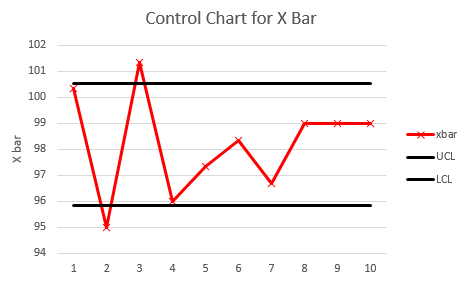
\includegraphics[scale=0.85]{xbarcontrol.png}\\
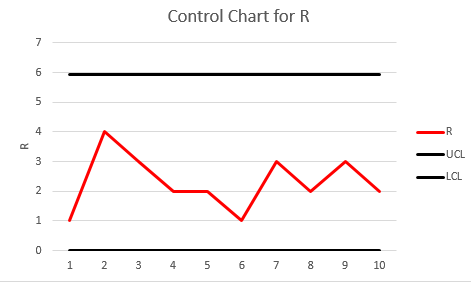
\includegraphics[scale=0.85]{rbarcontrol.png}
\end{center}
Here, we see that the $\bar{X}$ chart contains out of control points. This points to an ability to discriminate between different parts. Conversely, the $R$ control chart is within control. This shows us that the operator making the measurements is being consistent, a good sign. So, we consider the measurement error. We know that this error is normally distributed with variance$=\sigma^2_{gauge}$. Here, $\sigma^2_{gauge}=1.845618$.\\
Next, we compute $\sigma^2_{total}=4.717241$. Thus, we may compute,
\[\sigma_{prod}=\sqrt{\sigma_{total}^2-\sigma_{gauge}^2}=1.144961\]\\
Next, we compute the percent of variability of the gauge component, as,
\[\%Gauge=\frac{\sigma_{gauge}}{\sigma_{total}}=0.625499\]
Finally, we compute the $P/T$ ratio as,
\[P/T=\frac{6*1.358535}{115-85}=0.271707\]
Because $P/T>0.1$, we consider the gauge to be inadequate.
\item Using the data from problem 2, we compute the following, $\bar{X}_1=50.0333,\ \bar{X}_2=49.86667,\ R_1=1.7,\ R_2=2.3, \bar{R}=2$. From these basic descriptive statistics, we may now compute,
\begin{align*}
\sigma_{repeat} &= \frac{\bar{R}}{1.693}\\
&=1.181335\\
\sigma_{reprod} &= \frac{RANGE(\bar{X})}{1.128}\\
&=0.147754
\end{align*}
The standard deviation of measurement error is computed as,
\[\sigma_{MeasErr}=\sqrt{\sigma_{repeat}^2+\sigma_{reproduce}^2}=1.190539\]
Finally, we compute,
\[P/T=\frac{6*\sigma_{gauge}}{60-40}=0.3544\]
Since, $P/T>0.1$, the gauge is inadequate.
\item We consider the data in problem 3. As before, we compute the following,
\[\bar{X}=98.09375,\ \bar{R}=3.375\]
From this $\bar{X}$ and $R$ data, we construct the control charts as before,
\begin{center}
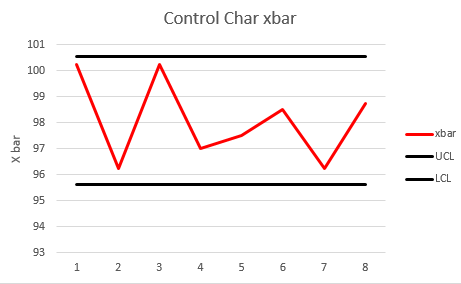
\includegraphics[scale=0.85]{xbarcontrol3.png}\\
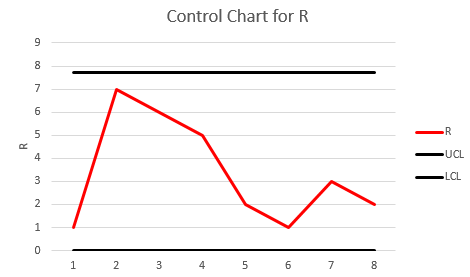
\includegraphics[scale=0.85]{rbarcontrol3.png}
\end{center}
From these plots, we see that the gauge has low discriminating power, but the operator has high consistency.\\
Next, we compute the total variability and product variability,
\[\sigma^2_{tot}=4.732863,\ \ \sigma^2_{prod}2.046066\]
Next, we compute,
\[\%Gauge=\frac{\sigma_{gauge}}{\sigma_{total}}=0.753452\]
Finally, we compute,
\[P/T=\frac{6*\sigma_{gauge}}{115-85}=0.327829\]
Since, $P/T>0.1$, the gauge is inadequate.
\item We compute with the new data, as before,
\[\sigma_{repeat}=1.279779,\ \ \sigma_{reprod}=0.689112\]
We expect that these variables are normally distributed with mean zero and variance from above.\\
Next, we compute the standard deviation of measurement error as,
\[\sigma_{MeasErr}=\sqrt{\sigma_{repeat}^2+\sigma_{reproduce}^2}=1.453517\]
Finally, we compute,
\[P/T=\frac{6*\sigma_{gauge}}{60-40}=0.383934\]
Since, $P/T>0.1$, the gauge is inadequate.
\end{enumerate}
\end{document}
